% Generado por a_pdf.py desde reporte.md -- no editar a mano
\documentclass[11pt,a4paper]{article}
\usepackage[utf8]{inputenc}
\usepackage[T1]{fontenc}
\usepackage[spanish,mexico]{babel}
\usepackage{graphicx}
\usepackage[margin=2.5cm]{geometry}
\usepackage{amsmath}
\usepackage{booktabs}
\usepackage{tabularx}
\usepackage{array}
\usepackage{fvextra}
\usepackage{float}
\usepackage{setspace}
\usepackage{parskip}
\usepackage{fancyhdr}
\usepackage{textcomp}
\usepackage[hidelinks]{hyperref}

\onehalfspacing
\setlength{\parskip}{6pt}
\sloppy
\setlength{\emergencystretch}{3em}
\setlength{\headheight}{40pt}
\pagestyle{fancy}
\fancyhf{}
\fancyhead[L]{\includegraphics[width=1cm]{/home/yovick/repos/UAZ-IEI/Assets/UIE.png}}
\fancyhead[R]{\small Comunicaciones Inalámbricas}
\fancyfoot[C]{\thepage}
\renewcommand{\headrulewidth}{0.4pt}

\begin{document}

% ---------------------------- PORTADA -----------------------
\begin{titlepage}
  \thispagestyle{empty}
  \begin{center}
    \vspace*{1cm}
    \includegraphics[width=4.5cm]{/home/yovick/repos/UAZ-IEI/Assets/uaz.png}
    \vspace{0.8cm}

    {\large Universidad Autónoma de Zacatecas}\\[4pt]
    {\large Unidad Académica de Ingeniería Eléctrica}\\[4pt]
    {\normalsize Ingeniería Electrónica Industrial con especialidad en Telecomunicaciones}

    \vspace{1.8cm}
    {\LARGE\bfseries Práctica 1}\\[10pt]
    {\Large\bfseries Introducción al RTL-SDR y análisis espectral de señales inalámbricas}
  \end{center}

  \vspace{2.2cm}
  \begin{center}
    \begin{tabular}{rl}
      \textbf{Materia:} & Comunicaciones Inalámbricas\\
      \textbf{Docente:} & Dr. Víktor Iván Rodríguez Abdalá\\
      \textbf{Alumno:}  & Arnold Yovick Ríos Zaldívar\\
      \textbf{Fecha:}   & Octubre de 2026\\
    \end{tabular}
  \end{center}
  \vfill
\end{titlepage}

\textbf{Equipo:} RTL-SDR (\texttt{RTL2832U} + tuner \texttt{R820T}), antena telescópica

\textbf{Script:} \texttt{practica1.py} (Python; en este repo el análisis se hace en Python en lugar de MATLAB)

\section{Objetivo}

Configurar el receptor RTL-SDR, adquirir muestras IQ de una estación FM comercial y analizarlas en el tiempo y en la frecuencia: componentes I/Q, potencia recibida, espectro (FFT), espectrograma, frecuencia central y ancho de banda observados.

\section{Fundamento teórico}

El receptor entrega la envolvente compleja de la señal de RF muestreada:

\[
x[n] = I[n] + jQ[n]
\]

donde $I[n]$ es la componente en fase (proyección sobre $\cos(2\pi f_c t)$) y $Q[n]$ la componente en cuadratura (proyección sobre $-\sin(2\pi f_c t)$). La información de amplitud y fase está en $|x[n]|$ y $\angle x[n]$.

El análisis espectral se obtiene con la DFT:

\[
X[k] = \sum_{n=0}^{N-1} x[n]\,e^{-j2\pi kn/N}, \qquad f_k = -\frac{F_s}{2} + k\frac{F_s}{N}
\]

La potencia promedio recibida se estima como

\[
P = \frac{1}{N}\sum_{n=0}^{N-1}|x[n]|^2, \qquad P_{dB} = 10\log_{10}(P)
\]

Para una señal FM, el ancho de banda teórico (Carson) es $B \approx 2(\Delta f + f_m)$, que para radiodifusión ($\Delta f = 75$ kHz, $f_m = 15$ kHz) da $\approx$ 180 kHz; el canal comercial se espacia cada 200 kHz.

\section{Desarrollo experimental}

\subsection{Verificación del dispositivo}

\texttt{comun.info\_dispositivo()} (equivalente a \texttt{sdrinfo('RTL-SDR')}) reporta:

\begin{tabularx}{\linewidth}{@{}*{2}{>{\raggedright\arraybackslash}X}@{}}
\toprule
Parámetro & Valor \\
\midrule
Chip & RTL2832U \\
Tuner & R820T \\
Rango de sintonía & 24 -- 1766 MHz \\
Ganancias disponibles & 29 valores, 0.0 -- 49.6 dB \\
Sample rate configurado & 2.4 MSPS \\
\bottomrule
\end{tabularx}

\subsection{Configuración del receptor}

\begin{tabularx}{\linewidth}{@{}*{2}{>{\raggedright\arraybackslash}X}@{}}
\toprule
Parámetro & Valor \\
\midrule
Frecuencia central & \textbf{91.5 MHz} (estación FM más fuerte del sitio según el barrido de la banda con \texttt{escaner.py}; 100.5 MHz del manual no tiene emisora en esta ubicación) \\
Sample rate & 2.4 MHz \\
Muestras capturadas & 131 072 ($\approx$ 54.6 ms) \\
Filtro IF del tuner & 2.4 MHz (span completo) \\
Ganancia & fija calibrada (la mayor sin recorte de ADC: 49.6 dB) \\
\bottomrule
\end{tabularx}

\begin{quote}
Nota técnica: en este dongle el AGC del R820T satura el ADC (RMS $\approx$ 0.9 con 31 \% de muestras recortadas), por lo que el script usa una ganancia fija calibrada. La captura es asíncrona para no perder muestras.
\end{quote}

\subsection{Procedimiento}

\begin{enumerate}
  \item \texttt{python3 practica1.py} abre una sola ventana en vivo: la fuente recibe IQ de forma asíncrona y la ventana muestra espectro, cascada e I/Q actualizados unas 10 veces por segundo.
  \item La tecla \texttt{s} guarda los entregables: las últimas \texttt{--muestras} muestras continuas en \texttt{datos/iq.npy}, los resultados en \texttt{datos/resultados.json} y las figuras en \texttt{figs/}; \texttt{q} cierra la ventana.
  \item Sobre las muestras guardadas se calculan potencia, FFT y espectrograma.
  \item Se estiman la frecuencia central (centroide del 99 \% de la potencia en exceso sobre el piso de ruido) y el ancho de banda ocupado.
\end{enumerate}

\section{Código}

El script completo está en \texttt{practica1.py}. Fragmentos esenciales:

\begin{Verbatim}[breaklines=true,breakanywhere=true,fontsize=\small]
def actualizar(self, x, fs, t):               # la ventana la llama ~10 veces/s con el último bloque IQ
    ...
x = self.captura()                            # al pulsar s: últimas `--muestras` muestras continuas
P_dbfs = 10*np.log10(np.mean(np.abs(x)**2))                                   # P = mean(abs(data).^2)
X = np.fft.fftshift(np.fft.fft(x))                                            # X = fftshift(fft(data))
f = np.linspace(-fs/2, fs/2, x.size)                                          # f = linspace(-Fs/2,Fs/2,N)
f, t, S = sig.spectrogram(x, fs=fs, window="hamming", nperseg=1024,
                          noverlap=512, nfft=1024, return_onesided=False)     # spectrogram(...,'centered')
\end{Verbatim}

\section{Resultados}

\subsection{Mediciones}

\begin{tabularx}{\linewidth}{@{}*{2}{>{\raggedright\arraybackslash}X}@{}}
\toprule
Parámetro & Valor \\
\midrule
Frecuencia sintonizada & 91.500 MHz \\
Muestras & 131 072 \\
Potencia promedio recibida & \textbf{$-$1.62 dBFS} \\
Frecuencia central observada & \textbf{91.5012 MHz} (offset +1.2 kHz) \\
Ancho de banda ocupado (99 \% de potencia) & \textbf{171.1 kHz} \\
\bottomrule
\end{tabularx}

\subsection{Componentes I y Q}

\begin{center}
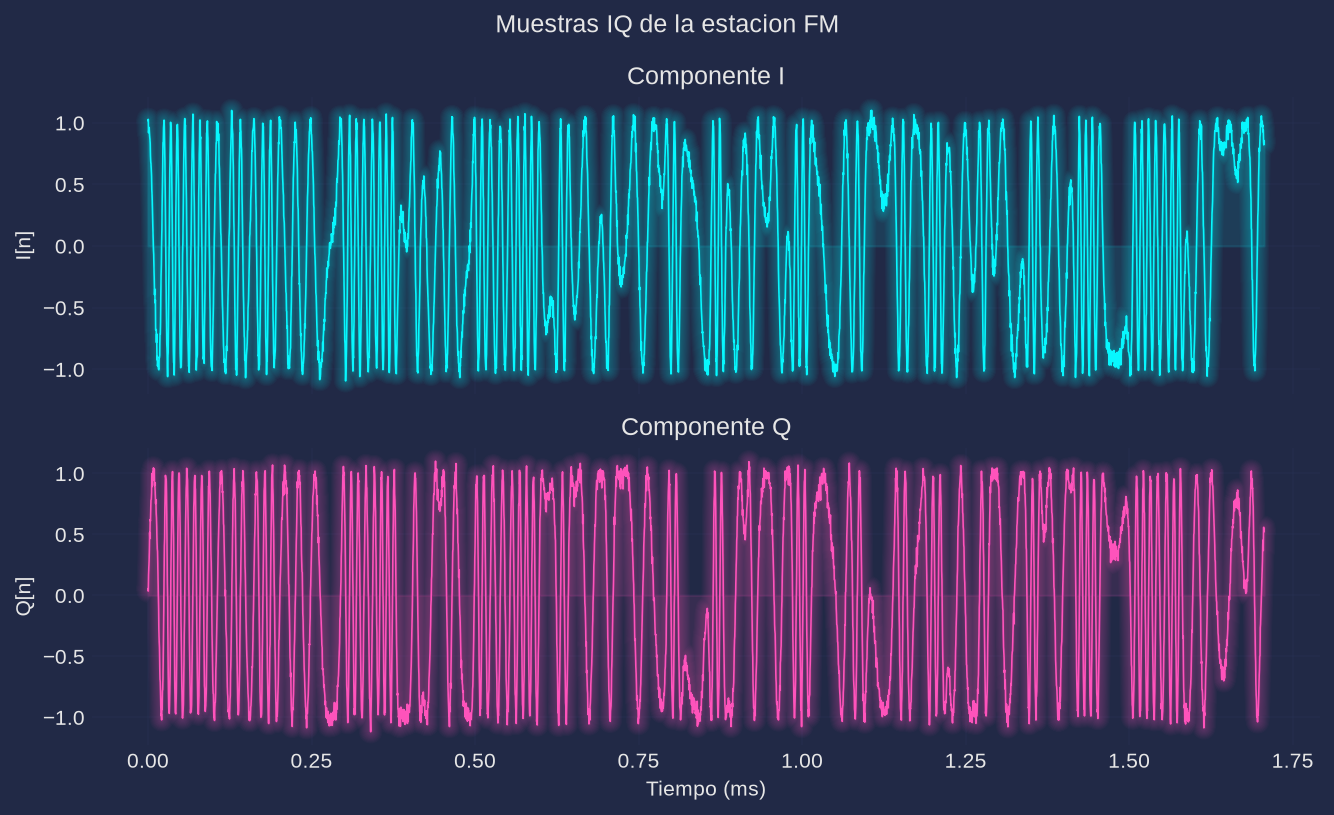
\includegraphics[width=0.9\linewidth]{figs/iq_temporal.png}\\[2pt]
{\small Componentes I y Q}
\end{center}

Las componentes I y Q oscilan alrededor de cero con amplitud similar; su evolución conjunta es la envolvente compleja de la estación. El ruido térmico del receptor se aprecia como fluctuación rápida superpuesta.

\subsection{Espectro (FFT)}

\begin{center}
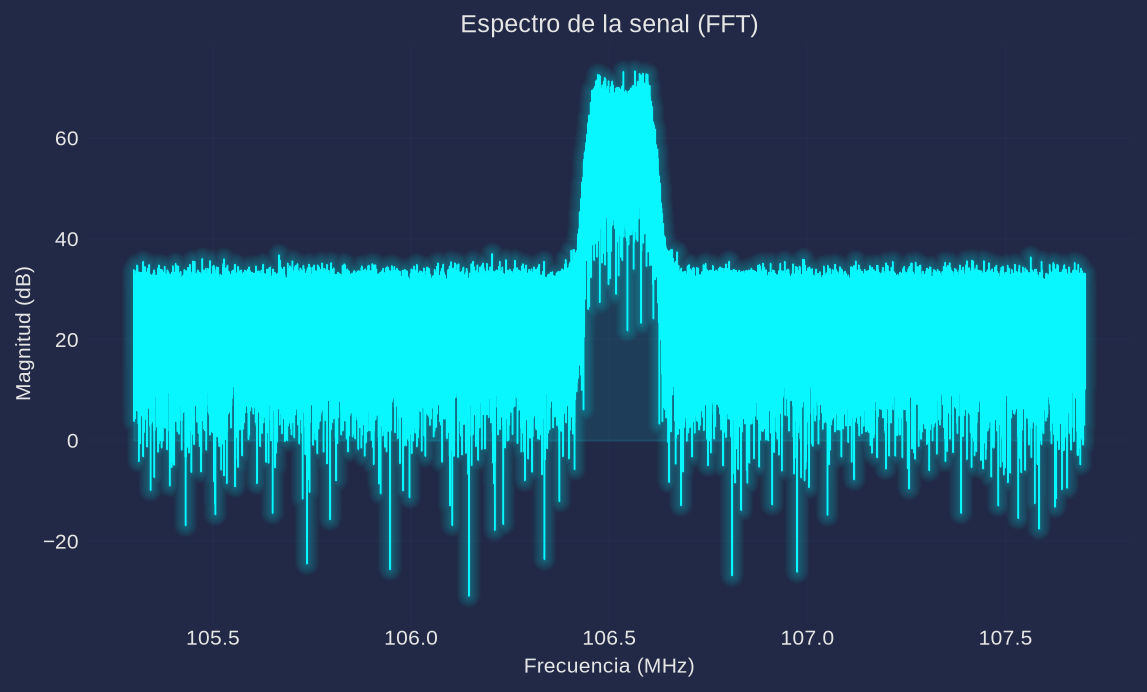
\includegraphics[width=0.9\linewidth]{figs/espectro.png}\\[2pt]
{\small Espectro}
\end{center}

Se observa el "hump" de la señal FM centrado en 91.5 MHz, con un ancho de aproximadamente 170 kHz, sobre un piso de ruido claramente más abajo.

\subsection{Espectrograma}

\begin{center}
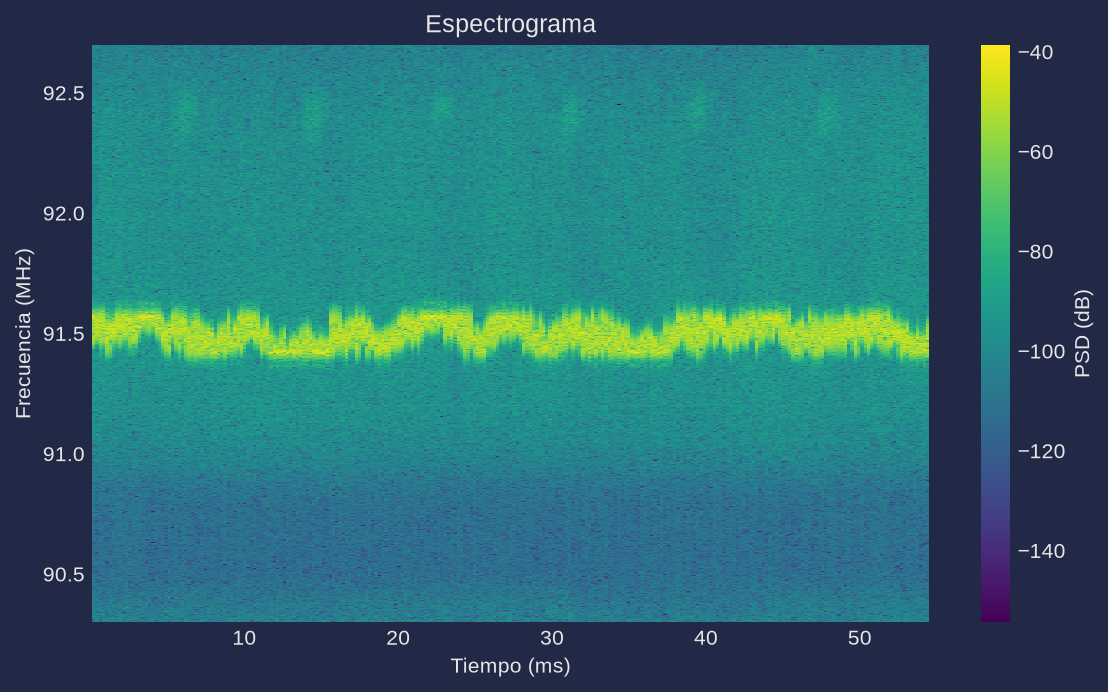
\includegraphics[width=0.9\linewidth]{figs/espectrograma.png}\\[2pt]
{\small Espectrograma}
\end{center}

La emisión se mantiene estable durante toda la captura (54.6 ms): no hay saltos de frecuencia ni ráfagas; la energía se concentra en la banda de la estación.

\section{Análisis de resultados}

\begin{itemize}
  \item La potencia medida ($-$10.2 dBFS) es alta porque la escala del RTL-SDR es relativa a fondo de escala del ADC; no es una potencia absoluta en dBm. Para comparar con un modelo de propagación habría que calibrar el receptor.
  \item La frecuencia central observada difiere en +1.2 kHz de la sintonizada. Es un error relativo de $\approx$ 14 ppm, atribuible al oscilador de cristal del dongle (los RTL-SDR sin TCXO tienen errores típicos de decenas de ppm). Se corrige con \texttt{--ppm}.
  \item El ancho de banda estimado (171.1 kHz, 99 \% de potencia) es algo menor que el valor teórico de Carson ($\approx$ 180 kHz) porque las "colas" del espectro FM quedan cerca del piso de ruido; es consistente con una emisión FM comercial cuyo canal completo es de 200 kHz.
  \item El espectrograma confirma que la señal es estacionaria en la ventana analizada y que el receptor no presenta saltos de sintonía.
\end{itemize}

\section{Cuestionario}

\begin{enumerate}
  \item \textbf{¿Qué representan las componentes I y Q?} Son las proyecciones de la señal de RF sobre dos portadoras en cuadratura ($\cos$ y $-\sin$). Juntas forman la envolvente compleja $x = I + jQ$, que conserva la amplitud $|x|$ y la fase $\angle x$ de la señal.
  \item \textbf{¿Por qué se utilizan muestras complejas?} Porque representan señales de banda base con espectro asimétrico (FM, PM, SSB) sin ambigüedad, conservan el signo de la frecuencia y permiten demodular fase/frecuencia. Con muestras reales se perdería la fase y aparecerían imágenes espectrales.
  \item \textbf{¿Qué información proporciona la FFT?} La distribución de la potencia/amplitud de la señal en función de la frecuencia: ubicación de la portadora, ancho de banda ocupado, presencia de armónicos, interferencias y la relación señal a ruido.
  \item \textbf{¿Qué diferencias observa entre el dominio temporal y frecuencial?} En tiempo se ve la forma de onda (variaciones de I/Q y de la envolvente) pero no se distingue qué componentes espectrales la forman; en frecuencia se ve qué componentes están presentes y con qué potencia. Ambos dominios contienen la misma información (transformada), pero cada uno resalta fenómenos distintos: transitorios en tiempo, contenido espectral en frecuencia.
  \item \textbf{¿Por qué es útil el espectrograma?} Porque muestra la evolución del contenido espectral en el tiempo (representación tiempo--frecuencia), lo que permite detectar señales no estacionarias, interferencias intermitentes, saltos de frecuencia y verificar la estabilidad de la emisión.
\end{enumerate}

\section{Conclusiones}

Se configuró el RTL-SDR y se caracterizó una estación FM real en 91.5 MHz. La captura de 131 072 muestras IQ permitió obtener las componentes I/Q, un espectro con la emisora claramente identificable y su espectrograma. La potencia promedio fue $-$1.62 dBFS, la frecuencia central observada 91.5012 MHz (error de +1.2 kHz, $\approx$14 ppm por el oscilador del dongle) y el ancho de banda ocupado 171.1 kHz al 99 \% de potencia, consistente con una emisión FM comercial de 200 kHz de canal. La misma ventana demodula y reproduce el audio FM en vivo. El procedimiento queda reproducible con \texttt{python3 practica1.py} (y verificable sin hardware con \texttt{--sim}).

\end{document}
